\documentclass[12pt]{article}

\usepackage[a4paper]{geometry}
\usepackage[utf8]{inputenc}
\usepackage[english]{babel}
\usepackage[automark]{scrpage2}
\usepackage{listings}
\usepackage{hyperref}
\usepackage{xcolor}
\usepackage{caption}
\usepackage{graphicx}

\pagestyle{scrheadings}
\clearscrheadfoot
\ihead[]{RoboSoccer Laboratory}
\ohead[]{Team C}
\cfoot[]{\pagemark}


\begin{document}

\section{Project Plan}
\subsection{Definition of Project Objectives}
The main project objective is winning the "\textsc{RoboSoccer} Championship" at the end of this course,
which requires both the implementation of low- and mid-level robot controls and an artificial intelligence with good tactics.

In addition the program has to obey the \textsc{RoboSoccer} rules during the match and has to have a penalty-shoot-out mode.

\subsection{Framework and Procedure}


\subsubsection*{Team Members}
\begin{itemize}
	\item Markus Hofbauer
	\item He Jiang
	\item Kevin Meyer
	\item Benedikt Schmidt
	\item Florian Wirnshofer
\end{itemize}

\subsubsection*{Team Organisation}
\begin{itemize}
	\item \textbf{Internal Communication}
	\begin{itemize}
		\item Team Discussion Board \\\mbox{(phpBB: \textit{https://forum.kevin-meyer.de})}
		\item Email
	\end{itemize}
	\item \textbf{Weekly Jour Fixe} at Laboratory or Eikon
	\item Additional meetings on demand
\end{itemize}

\subsubsection*{Hardware}
Each team controls three  \textsc{Pololu 3pi} robots with the purpose of shooting a golf ball into the goal of the enemy.
The robots are connected to a real-time server via \textsc{Bluetooth} and located using a \textsc{FireWire} camera above the playground.

\subsubsection*{Software}
\begin{itemize}
	\item \textbf{Target and Development-OS:} Linux
	\item \textbf{IDE:} Qt Creator
	\item \textbf{VCS:} Git (hosted on \textit{bitbucket.org})
	\item \textbf{Build System:} CMake
\end{itemize}

\subsection{Tasks}
The project strategy is based on the spiral model with the following milestones:
\begin{itemize}
	\item \textbf{Deadline: \textcolor{red}{07.05.2014}}
	\begin{itemize}
		\item Kickoff Position
		\item Goalkeeper
		\item Penalty Shooting
	\end{itemize}
	
	\item \textbf{Deadline: \textcolor{red}{04.06.2014}}
	\begin{itemize}
		\item Collision Avoidance
		\item Ball Control
		\item Player Interaction
	\end{itemize}
	
	\item \textbf{Strategy and Tactics}\\
	\textbf{Deadline: \textcolor{red}{25.06.2014}}
	
	\item \textbf{\textsc{RoboSoccer} Championship}\\
	\textbf{Deadline: \textcolor{red}{02.07.2014}}
\end{itemize}

\subsection{Resource Plan}
In addition to the standard responsibilities, every team member is responsible for special tasks:
\begin{itemize}
	\item \textbf{PM:} Benedikt Schmidt
	\begin{itemize}
		\item Communication with the contact person and the tutor of the course
		\item General team coordination
		\item Monitor realization of project plan
	\end{itemize}
	 
	\item \textbf{QM:} Florian Wirnshofer
	\begin{itemize}
		\item Ensure sufficient unit tests
		\item Continuous testing on hardware
		\item Balance quality aspiration and effort
	\end{itemize}
	
	\item \textbf{CM:} Kevin Meyer
	\begin{itemize}
		\item Ensure self-explaining and readable code style
		\item Supervise the documentation
		\item Maintain repository and discussion board
	\end{itemize}
	
	\item \textbf{SD:} Markus Hofbauer, He Jiang 
	\begin{itemize}
		\item Design and verify code structure
		\item Ensure building code
		\item Choose and connect external libraries
	\end{itemize}
	
\end{itemize}

\subsection{Cost Plan}
In every Jour Fixe the team will discuss and create implementation issues, which are listed and managed inside bitbucket's issue tracker. 
Each team member will try to complete his assigned issues until the next Jour Fixe and report about it.

This approach will strengthen each team member's knowledge concerning the current project status and will provide a general insight on all project tasks. As a consequence of this benefit, scaling the effort needed for individual tasks will only be a small issue compared to estimating the effort of individual tasks at project start.

\subsection{Implementation}
Class diagramm: First draft\\
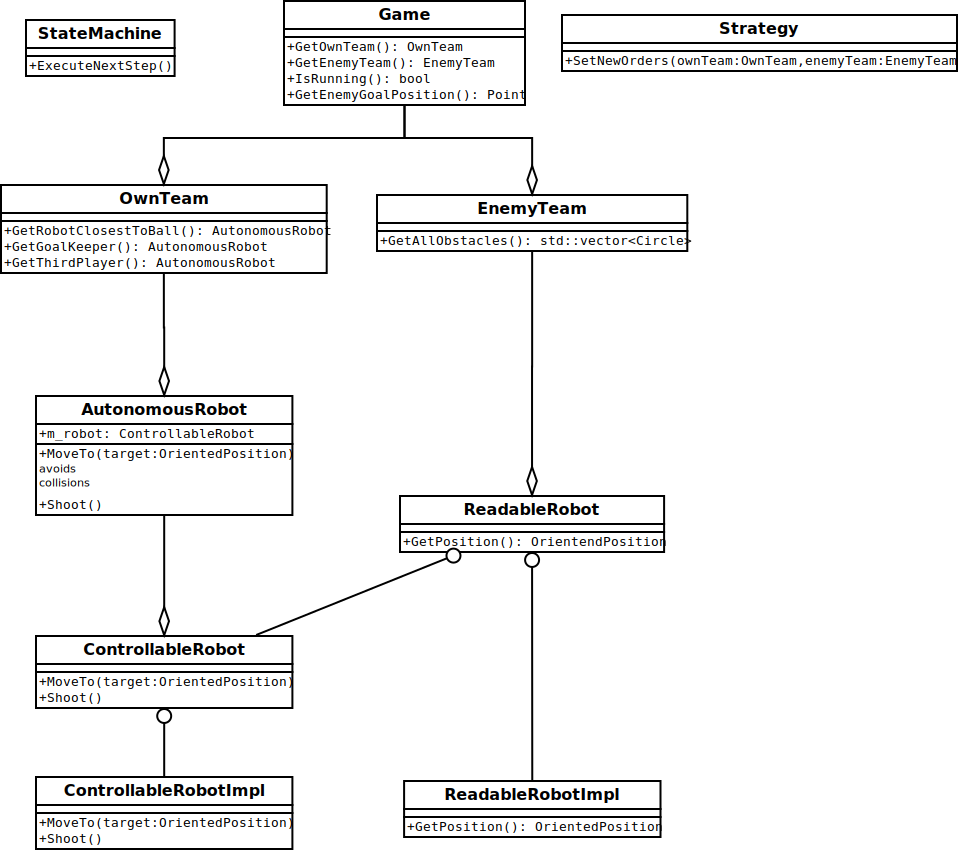
\includegraphics[width=\textwidth]{../architecture.pdf}
\subsection{Time Schedule}
% Split Gantt Chart into two pieces: 
% 21.04.14 - 25.05.14
% 26.05.14 - 29.06.14
\centering
\includegraphics[width = 1.3\textwidth , angle = 270]{../ganttchart1.png}
\includegraphics[width = 1.3\textwidth , angle = 270]{../ganttchart2.png}

\end{document}
